\chapter{Experiments and Results}\label{ch4:experiments-results}

In this chapter, we present some quantitative and qualitative evaluations of the variants of the recreated single-view MPI model retrained on different combinations of the MannequinChallenge and RealEstate10K datasets. We use the pretrained weights of the single-view MPI model as the benchmark and compare the abilities of all model variants at hand to generate novel views. We adopt some of the quantitative metrics from Tucker and Snavely's single-view MPI paper~\cite{single_view_mpi} --- PSNR, SSMI~\cite{wang_image_2004}, and LPIPS~\cite{zhang_unreasonable_2018} --- to give numeric values to the similarities between MPI-rendered video frames and the corresponding ground truth target frames the rendering process attempts to replicate.

The model variants used to compute the metrics stated above are characterized by the following hyperparameters/metadata: ---
\begin{itemize}
    \item Depth loss weight, as explained in subsection~\ref{subsec:base-papers}.
    \item The number of disparity map channels specified in the \texttt{tf.function} input signature for the bilinear sampling function, \texttt{sample\_disparities(disparity,\\points)}, involving the predicted disparity and the input visible points.
    \item The lower bound on the number of visible points allowed per frame. Videos with even one frame having points below this threshold would be removed from training.
    \item The choice of datasets used to train on --- MannequinChallenge, RealEstate10K, or both.
    \item Whether multiple GPU workers were engaged or not.
\end{itemize}
Even seemingly innocuous hyperparameter values such as those for the number of disparity map channels specified, we believe, could have easily held sway over training progress. Pitting these variants against each other in terms of the three computed metrics helped us select the best variant to simulate one half of a video chat with.

% \begin{figure}[!h]
%     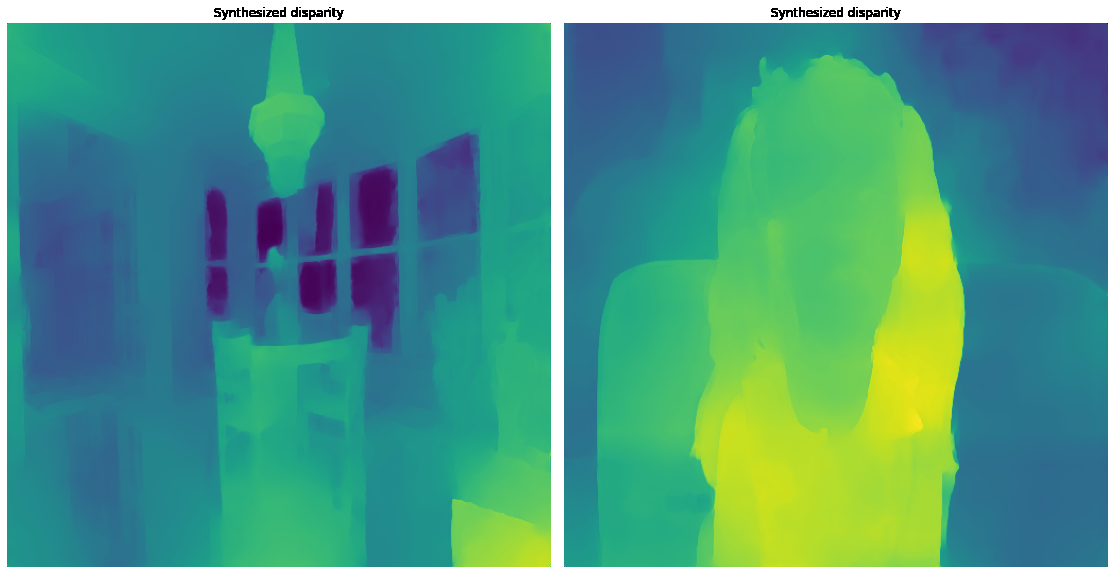
\includegraphics[width=1\columnwidth]{figures/great-off-kilter-disparity.png}
%     \caption{Training Loss}
%     \label{fig:training-loss}
%     {\small }  
% \end{figure}

\begin{figure}[!h]
    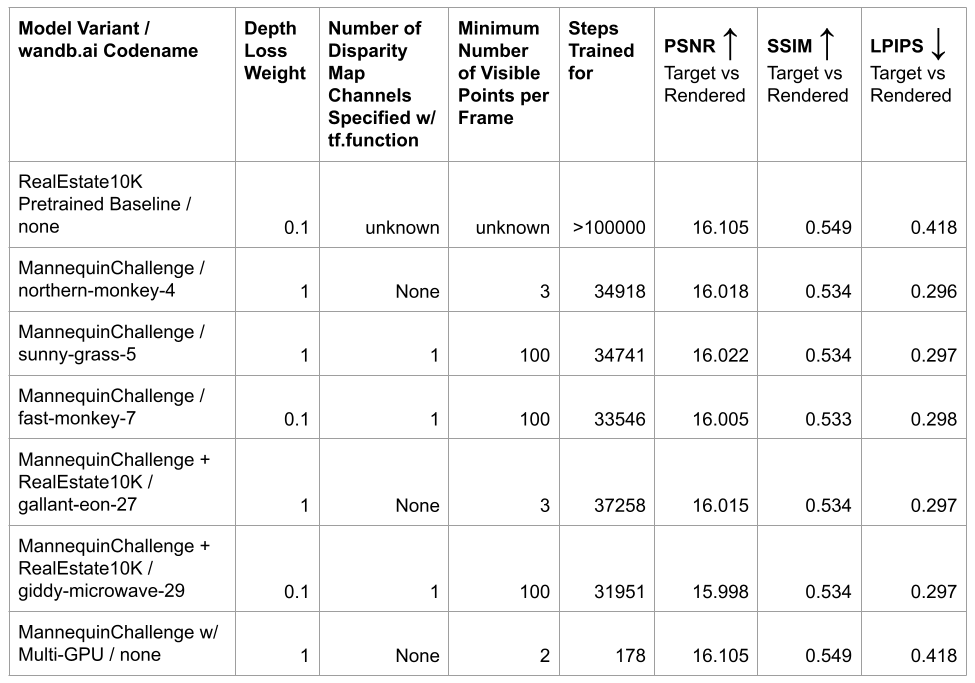
\includegraphics[width=1\columnwidth]{figures/model-variants-metrics.png}
    \caption{Model Variants' PSNR, SSIM, and LPIPS evaluations}
    \label{fig:model-variants-metrics}
    {\small }  
\end{figure}

We sifted through the test set of the MannequinChallenge dataset to hand pick a set of 333 videos that contained ORB-SLAM2-curated sequences\footnote{the timestamp, camera intrinsics and extrinsics of all frames of each of which are listed in the corresponding text files in the dataset} which had video-chat-relevant features such as the heads and torsos of people being focused on rather than having wide shots of entire bodies, the number of people in the frame being mostly limited to one or two as opposed to multiple people being featured, and the head pose of people being roughly or even very loosely aligned with the camera (there was hardly anybody that looked directly at the camera). We put them in the \texttt{test-yes/} bin. We also curated \texttt{test-maybe/} (311 videos) and \texttt{test-no/} (25 videos) bins that consisted of the rest of the MannequinChallenge test set with sequences either having no relevance to video chat (like there being hardly anyone in the frames) for \texttt{test-no/} to those falling heavily in the gray areas between \texttt{test-yes/} and \texttt{test-no/} for \texttt{test-maybe/}. We even occasionally interspersed the \texttt{test-yes/} and \texttt{test-maybe/} bins with videos containing sequences that portrayed people facing diametrically opposite the camera, just to really challenge the model variant being tested.

Of the various aspects of the code that we modelled from the textual descriptions and relevant code snippets obtained from both the single-view and stereo MPI papers such as \texttt{generator\_test.py}, \texttt{generator\_train.py}, \texttt{data\_loader.py}, \texttt{train.py}, and \texttt{test.py}, the scripts relevant to the experiments in this section are \texttt{test.py} and \texttt{generator\_test.py} (Section~\ref{sec:code-sources}). For testing, the generator first aggregates all videos names from the directory input to it and for each of these, it picks \texttt{reference\_image} and \texttt{target\_image} to be either 5 or 10 frames apart. \texttt{reference\_image} is the frame that \texttt{test.py} uses to infer the MPI of the scene from and \texttt{target\_image} is supposedly a view of the same scene from a different angle. The possibility that, when the camera moves from one scene to another in the same video, \texttt{reference\_image} may depict a scene different from the one captured by \texttt{target\_image} is expected to be extremely rare as both datasets have been curated by similar ORB-SLAM2 and COLMAP processes. In such hypothetical cases, \texttt{target\_image} will be erroneously rendered by \texttt{mpi.render} in \texttt{rendered\_image}. But since we take the mean of the computed metrics over hundreds of \texttt{test.py} processed \texttt{reference\_image}, \texttt{target\_image} pairs, we believe the final accuracies of a variant's mean metrics will not be off the tracks much and that they shall still be used to determine a variant’s performance satisfactorily. Each of the three metrics are calculated between \texttt{target\_image} and \texttt{rendered\_image}. We first test and compute metrics of frames 5 part and then we repeat the same test process for frames 10 apart just to show (as in the case of the single-view MPI paper) that the longer the baseline between reference/source and target views, the less the accuracy will be of the rendered image. Moreover, we also calculate the metrics for all processed \texttt{(reference\_image, target\_image)} pairs, to catch the hypothetical anomalies of the complete scene changes mentioned above. 

We also took an interesting detour in our project when we attempted to parallelize training across multiple GPUs, which we believed would allow us to increase the batch size\footnote{currently limited to 4 pairs of reference and target images and their respective camera poses and intrinsics, along with the 3D points of the reference image} and thereby let larger parts of our 60000+ training ready sequences with associated point clouds be used for learning by our recreated model. This would assist the model in avoiding local minima and maxima. But, since TensorFlow's direct conversion procedure that would let standard single-GPU-utilizing scripts become multi-GPU-faring is as yet still an evolving process requiring careful attention to resource allocation issues among the various replicas of the parallelizable aspects of the model\footnote{such as the dataset generator, the loss functions aggregator, etc.} spread across GPUs, our training got undercut after a good start by a resource exhaustion error at training step 178. Nevertheless, we computed all three metrics for this other model variant retrained on MannequinChallenge data using \texttt{tf.distribute.MirroredStrategy}, and capable of harnessing the power of multiple GPUs.

The rest of this chapter presents the results for the experiments done on the baseline pretrained model and the variant retrained on only the video-chat-relevant MannequinChallenge dataset. Currently, our \texttt{generator\_test.py} is only able to pick random pairs of reference and target frames from the 333 \texttt{test-yes/} videos. Sequential pair picking, would avoid possible repetition of selected pairs and allow for an exhaustive coverage of the test set. We also note that given that even the smaller of the two datasets has 100,000+ frames and we have not even gone to 50,000 steps of training for any model variant\footnote{the loss become less than 1 and stagnates sooner than 50,000 steps (Figure~\ref{fig:training-loss})}, it is not very like that the training process may see the same frame twice. So, perhaps, computing the evaluation metrics on the training data can double in for doing the same for validation data itself, even though we haven't set aside validation data. As for the metrics, an LPIPS value of 0 indicates there is either a perfect match between the images being compared or the images being compared are one and the same. On the contrary, SSIM values of 1 indicate a perfect match. Both these metrics range from 0 to 1. PSNR values, measured in decibels (dB), don't generally have an upper limit but values 20 dB or higher are considered acceptable. In calibrating our implementations of these metrics, when we compared an image with itself, we found the mean LPIPS, SSIM and PSNR values over 300 images to be close to 0, 1, and higher than 30, respectively.

The authors of single-view MPI paper used the following pointers to qualitatively compare the discrepancies in the results generated by each variant model: (i) handling of occluded content, (ii) unpleasant artifacts at the edges of foreground objects. In addition to visually checking for these, we find that visually checking the disparity map is also useful in verifying the quality of the MPI produced.  

The metrics' mean value tables presented in this chapter, produced via the random \texttt{(reference\_image, target\_image)} pair experiments so far validate one of the hypotheses of this thesis by showing that transfer learning with completely unfrozen layers seems to be helping the single-view MPI pick up from where it left off by specializing and improve upon its performance in accurately predicting close up shots of people in video-chat-relevant frames. 

A further testimony to this improvement can be obtained by inspecting the performance of even the prematurely halted multi-GPU variant. It performs at par with the original pretrained model which indicates that the pretrained model has begun to continue where it left off and specialize in processing video-chat-like frames. It would have run properly if not for the resource errors mentioned in the earlier that could point to underlying issues like possible unchecked growth of TensorFlow graphs per pipeline replica or such. This seems to be the case even though the replicas seem to be getting properly allocated inputs and their respective outputs also seem to be getting well gelled together in the end.

The authors of the single-view MPI paper used pointers like the handling of occluded content, the production of unpleasant artifacts at the edges of foreground objects, and so on to qualitatively compare the discrepancies in the results generated by each variant model. In addition to visually checking for these, we, like the authors also found that visually checking the disparity maps is also useful in verifying the quality of the MPI produced.

% We refer to the qualitative results present in this chapter. To cap it off with the help of OpenFace 2.2, we also include a few snapshots of how a rerendered frames vary with changes in head pose in figure~\ref{fig:rerendered-with-openface}.  

% As the girl looks to the left the opposite concurrent video frame moves to the right and vice versa
% Please head over to the github repo for this project to observe videos of simultaneous changes simulating a two way video chat.

% \begin{figure}[!h]
%     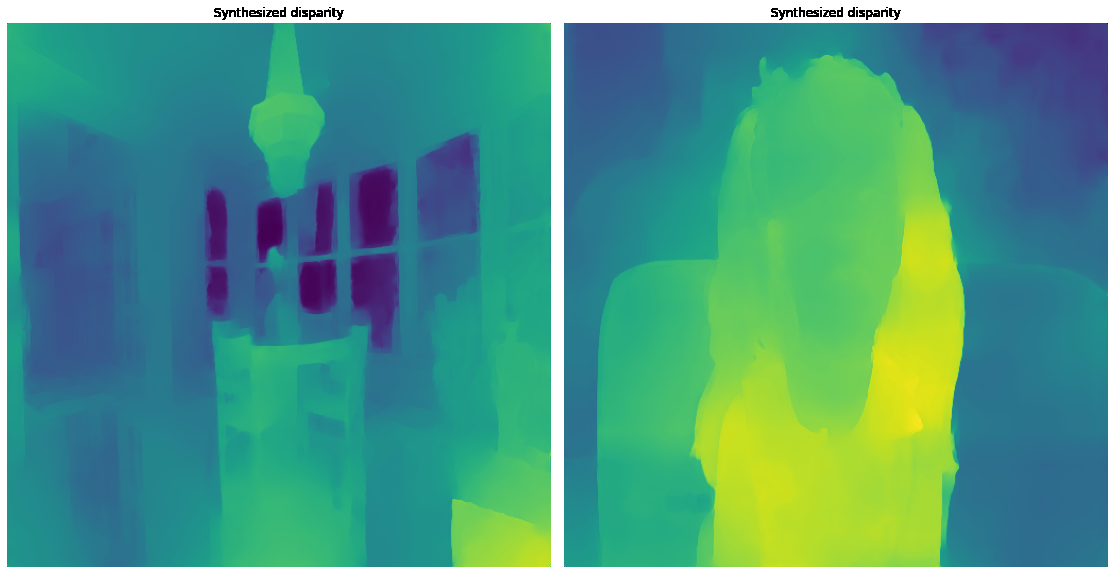
\includegraphics[width=1\columnwidth]{figures/great-off-kilter-disparity.png}
%     \caption{Rerendered frames varying with changes in head pose}
%     \label{fig:rerendered-with-openface}
%     {\small }  
% \end{figure}

\begin{figure}[!h]
\begin{tabular}{cccc}
\subfloat[reference]{\includegraphics[width = 1.3in]{figures/pretrained-5-apt/000000_image_reference.png}} &
\subfloat[target]{\includegraphics[width = 1.3in]{figures/pretrained-5-apt/000000_image_target.png}} &
\subfloat[disparity]{\includegraphics[width = 1.3in]{figures/pretrained-5-apt/000000_image_disparity.png}} &
\subfloat[rendered]{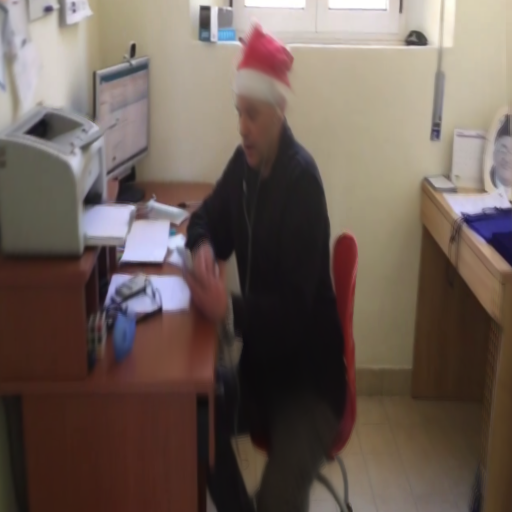
\includegraphics[width = 1.3in]{figures/pretrained-5-apt/000000_image_render.png}}\\
\subfloat[reference]{\includegraphics[width = 1.3in]{figures/mann-1841-5-apt/000000_image_reference.png}} &
\subfloat[target]{\includegraphics[width = 1.3in]{figures/mann-1841-5-apt/000000_image_target.png}} &
\subfloat[disparity]{\includegraphics[width = 1.3in]{figures/mann-1841-5-apt/000000_image_disparity.png}} &
\subfloat[rendered]{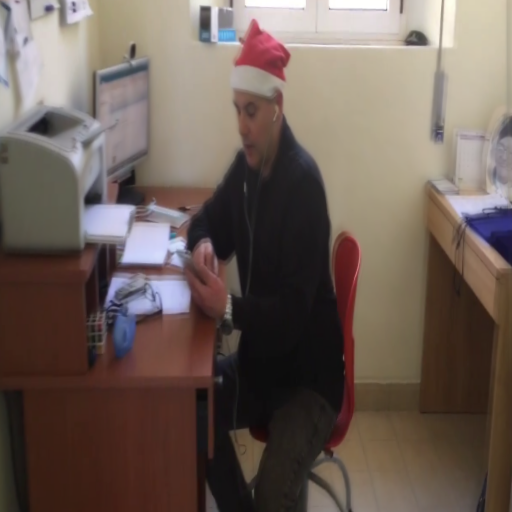
\includegraphics[width = 1.3in]{figures/mann-1841-5-apt/000000_image_render.png}}\\
\subfloat[reference]{\includegraphics[width = 1.3in]{figures/pretrained-10-apt/000000_image_reference.png}} &
\subfloat[target]{\includegraphics[width = 1.3in]{figures/pretrained-10-apt/000000_image_target.png}} &
\subfloat[disparity]{\includegraphics[width = 1.3in]{figures/pretrained-10-apt/000000_image_disparity.png}} &
\subfloat[rendered]{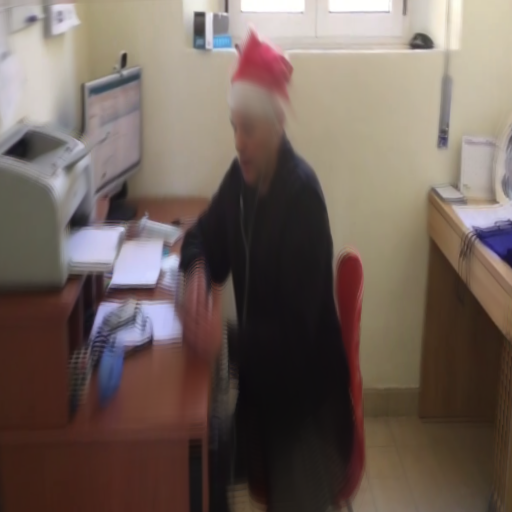
\includegraphics[width = 1.3in]{figures/pretrained-10-apt/000000_image_render.png}}\\
\subfloat[reference]{\includegraphics[width = 1.3in]{figures/mann-1841-10-apt/000000_image_reference.png}} &
\subfloat[target]{\includegraphics[width = 1.3in]{figures/mann-1841-10-apt/000000_image_target.png}} &
\subfloat[disparity]{\includegraphics[width = 1.3in]{figures/mann-1841-10-apt/000000_image_disparity.png}} &
\subfloat[rendered]{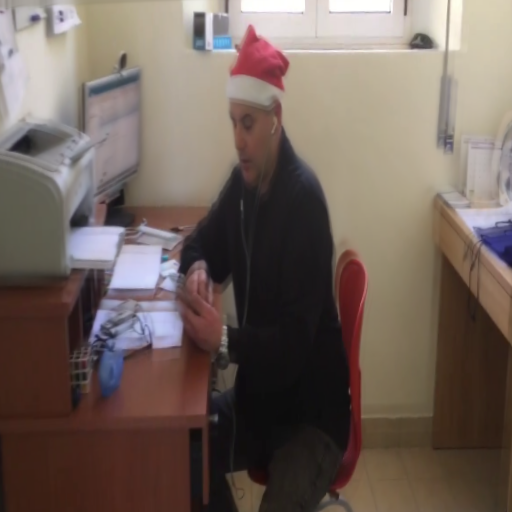
\includegraphics[width = 1.3in]{figures/mann-1841-10-apt/000000_image_render.png}}
\end{tabular}
\caption{Model Variants' Output Visualizations}
    {\small First Row: Pretrained Model -- tested 5 frames apart; Second Row: Retrained Model -- trained on 1841 Mannequin Challenge videos -- tested 5 frames apart; Third Row: Pretrained Model -- tested 10 frames apart; Fourth Row: Retrained Model -- trained on 1841 Mannequin Challenge videos -- tested 10 frames apart}
\end{figure}